\documentclass[UTF8]{article}
\usepackage{ctex}
\usepackage{amsmath}
\usepackage{graphicx}
\usepackage{listings}
\usepackage{color}
\usepackage{geometry}
\usepackage{caption}
\usepackage[dvipsnames]{xcolor} % 更全的色系
\usepackage{listings} % 排代码用的宏包
\usepackage{svg}
\usepackage{subcaption}
\usepackage{hyperref}
% Page layout
\geometry{a4paper, margin=1in}

% Title and Author
\title{Chapter 4 频域图像增强}
\author{李想 \quad P12214061}

\begin{document}

\maketitle

% \tableofcontents
% \newpage
\section{问题一}
选取两张图像,分别进行傅里叶变换,计算并显示其幅度谱和相位谱。如图\ref{fig:figures}所示:
% 导言区需添加:
% \usepackage{graphicx}
% \usepackage{subcaption}

\begin{figure}[htbp]
    \centering
    \begin{subfigure}{0.4\textwidth}
      \centering
      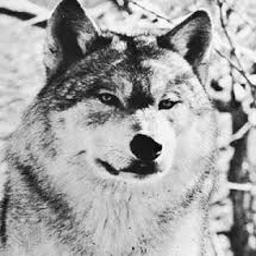
\includegraphics[width=0.6\textwidth]{../img/img1_1.jpg}
      \caption{img1}
      \label{fig:subfig1} % 规范命名
    \end{subfigure}
    \hfill
    \begin{subfigure}{0.4\textwidth}
      \centering
      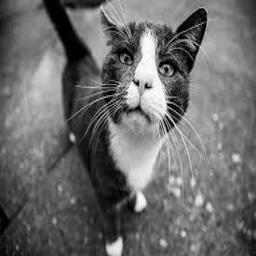
\includegraphics[width=0.6\textwidth]{../img/img2_1.jpg}
      \caption{img2}
      \label{fig:subfig2} % 规范命名
    \end{subfigure}
    \caption{原始图像}
    \label{fig:figures} % 主图标签保持原样
  \end{figure}
  
  % 正文中引用示例:
  % 子图~\ref{fig:subfig1} 和~\ref{fig:subfig2} 位于图~\ref{fig:figures} 中。
\par 对图像进行傅里叶变换后,通过ifftshift函数将频谱中心化,两张图像的幅度谱和相位谱分别如图二所示:
\begin{figure}[htbp]
    \centering
    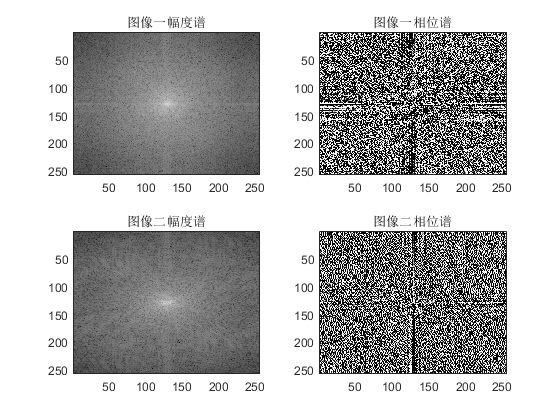
\includegraphics[width=0.6\textwidth]{../img/A-P.png} % Replace with your image file
    \caption{原始图像的幅度谱和相位谱}
    \label{fig:AP}
\end{figure}
\par 交换两张图像的幅度谱和相位谱后,去中心化并进行傅里叶逆变换,得到的图像如图三所示:
\begin{figure}[htbp]
    \centering
    \begin{subfigure}{0.4\textwidth}
        \centering
        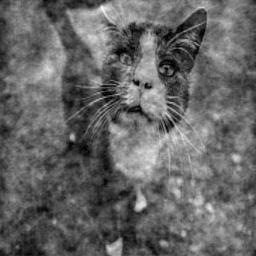
\includegraphics[width=0.6\textwidth]{../img/img1_2.jpg} % Replace with your image file
        \caption{交换幅度谱后的图\ref{fig:subfig1}}
        % \label{fig:first}
    \end{subfigure}
    \hfill
    \begin{subfigure}{0.4\textwidth}
        \centering
        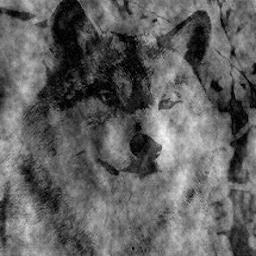
\includegraphics[width=0.6\textwidth]{../img/img2_2.jpg}
        \caption{交换相位谱后的图\ref{fig:subfig2}}
        % \label{fig:second}
    \end{subfigure}        
    \caption{交换幅度谱和相位谱后的图像}
    % \label{fig:figures}
\end{figure}
\newpage 实验结果显示相位信息决定了图像中物体的空间位置、边缘轮廓和结构布局等信息,而幅度信息则决定了图像的亮度、对比度和纹理等信息。
通过交换幅度谱和相位谱,我们可以看到图像的结构和纹理发生了明显的变化,图一\ref{fig:subfig1}为一只狗,交换相位后看起来更像一只猫,
说明相位谱在图像中起着重要的作用。即使完全替换幅度,只要保持相位不变,图像的基本结构仍可辨认。
\section{问题二}
非均匀光照条件下的图像常因亮度分布不均导致细节丢失,影响后续分析与应用。
本实验通过同态滤波方法,在频域中分离图像的光照分量与反射分量,实现了对非均匀背景的亮度矫正与细节增强。
\subsection{成像模型}
图像形成过程可建模为:
\begin{equation}
    f(x,y) = i(x,y) \cdot r(x,y)
\end{equation}
其中:
\begin{itemize}
    \item $i(x,y)$:低频光照分量
    \item $r(x,y)$:高频反射分量
\end{itemize}

\subsection{同态滤波原理}
通过以下变换实现分量分离:
\begin{align}
    \ln f(x,y) &= \ln i(x,y) + \ln r(x,y) \\
    Z(u,v) &= H(u,v) \cdot \mathcal{F}[\ln f(x,y)] \\
    g(x,y) &= \exp\left( \mathcal{F}^{-1}[Z(u,v)] \right)
\end{align}

\subsection{高斯滤波器设计}
采用频域高斯响应函数:
\begin{equation}
    H(u,v) = (\alpha_H - \alpha_L)(1 - e^{-D^2(u,v)/d^2}) + \alpha_L
\end{equation}
其中参数定义:
\begin{itemize}
    \item $D(u,v)$: 频域点到中心的欧氏距离
    \item $d=20$: 截止频率
    \item $\alpha_L=0.5$: 低频抑制系数
    \item $\alpha_H=1.2$: 高频增强系数
\end{itemize}
高斯滤波器如图\ref{fig:gaussian}所示:
\begin{figure}[htbp]
    \centering
    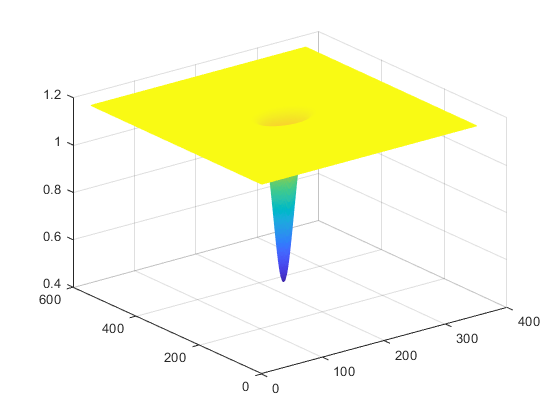
\includegraphics[width=0.5\textwidth]{../img/filter.png} % Replace with your image file
    \caption{高斯滤波器}
    \label{fig:gaussian}
\end{figure}
\subsection{同态滤波处理}
同态滤波增强后的图像如图\ref{fig:homo}所示:
\begin{figure}[htbp]
    \centering
    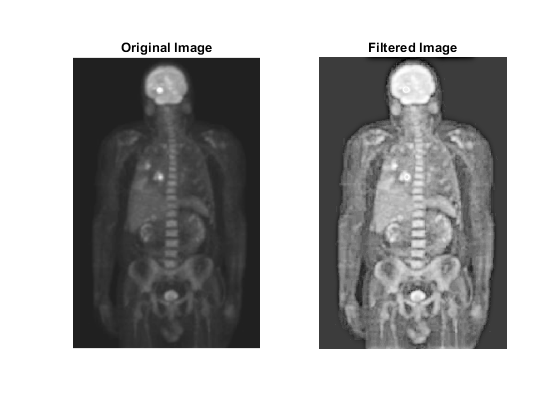
\includegraphics[width=0.6\textwidth]{../img/homo.png} % Replace with your image file
    \caption{同态滤波增强图像}
    \label{fig:homo}
\end{figure}
\par 观察滤波后的图像可以发现图像对比度增强,可以清晰的展现低灰度的部分,
高频分量增强,图像被锐化,轮廓更明显。
\end{document}